% Copyright 2004 by Till Tantau <tantau@users.sourceforge.net>.
%
% In principle, this file can be redistributed and/or modified under
% the terms of the GNU Public License, version 2.
%
% However, this file is supposed to be a template to be modified
% for your own needs. For this reason, if you use this file as a
% template and not specifically distribute it as part of a another
% package/program, I grant the extra permission to freely copy and
% modify this file as you see fit and even to delete this copyright
% notice. 

\documentclass{beamer}

% There are many different themes available for Beamer. A comprehensive
% list with examples is given here:
% http://deic.uab.es/~iblanes/beamer_gallery/index_by_theme.html
% You can uncomment the themes below if you would like to use a different
% one:
%\usetheme{AnnArbor}
%\usetheme{Antibes}
%\usetheme{Bergen}
%\usetheme{Berkeley}
%\usetheme{Berlin}
%\usetheme{Boadilla}
%\usetheme{boxes}
%\usetheme{CambridgeUS}
%\usetheme{Copenhagen}
%\usetheme{Darmstadt}
%\usetheme{default}
%\usetheme{Frankfurt}
%\usetheme{Goettingen}
%\usetheme{Hannover}
%\usetheme{Ilmenau}
%\usetheme{JuanLesPins}
%\usetheme{Luebeck}
\usetheme{Madrid}
%\usetheme{Malmoe}
%\usetheme{Marburg}
%\usetheme{Montpellier}
%\usetheme{PaloAlto}
%\usetheme{Pittsburgh}
%\usetheme{Rochester}
%\usetheme{Singapore}
%\usetheme{Szeged}
%\usetheme{Warsaw}

\usepackage[utf8]{inputenc} 
\usepackage[T1]{fontenc}
\usepackage{setspace}

\usepackage{listings}
\usepackage{color}

\title[AIAYN]{Attention is All You Need}

\author{Andrew Drozdov}

% Let's get started
\begin{document}

% Title
\begin{frame}
  \titlepage
\end{frame}
%

% What?
\begin{frame}{What?}{}
\centering
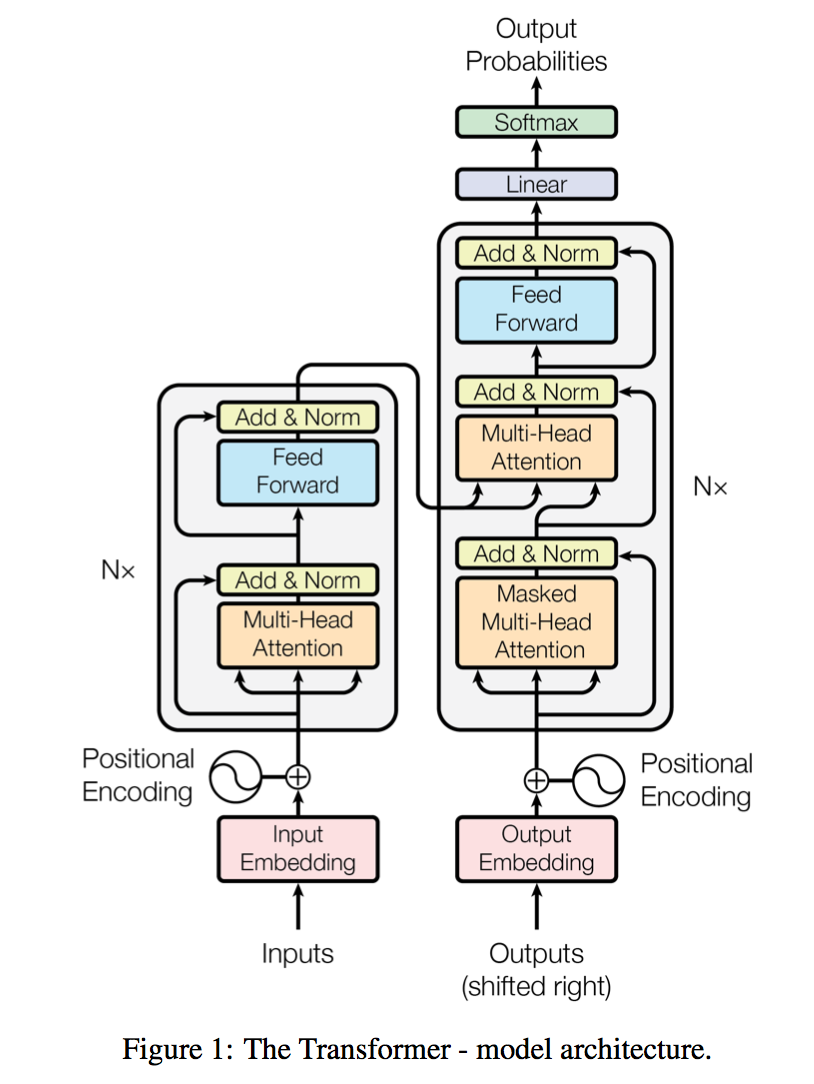
\includegraphics[width=0.5\textwidth]{img/transformer.png}
\end{frame}
%

% Why? (Architecture Perspective)
\begin{frame}{Why? (Architecture Perspective)}{}
\begin{itemize}
\item Many NLP tasks have SotA set by LSTM or GRU, models with sequential dependencies making them difficult to paralellize.

\item There are other popular architectures lately:
\begin{itemize}
\item QRNN \footnote[frame]{\url{https://www.salesforce.com/products/einstein/ai-research/neural-network-building-block-accurate-understanding/}} / SRU \footnote[frame]{\url{https://github.com/taolei87/sru}}
\item CNN  \footnote[frame]{\url{https://github.com/facebookresearch/fairseq}}
\end{itemize}
\item[] But they still usually have some sequential dependencies.

\item The model in AIAYN has no sequential dependencies.

\item Attention-only model does exist, but not for decoding.

\end{itemize}
\end{frame}
%

% Why? (Performance Perspective)
\begin{frame}{Why? (Performance Perspective)}{}
\begin{itemize}
\item Transformer Network can be used for many tasks:
\begin{itemize}
\item WMT 14 (En to Ge). 28.4 BLEU (+2)
\item WMT 14 (En to Fr). 41.0 BLEU (single model, fast/easy to train)
\item Constituency Parsing
\end{itemize}

\item[] Some of these numbers are more impressive than seen in some similar papers.

\end{itemize}
\end{frame}
%

% Background (RNNs)
\begin{frame}{Background (RNNs)}{}
\centering
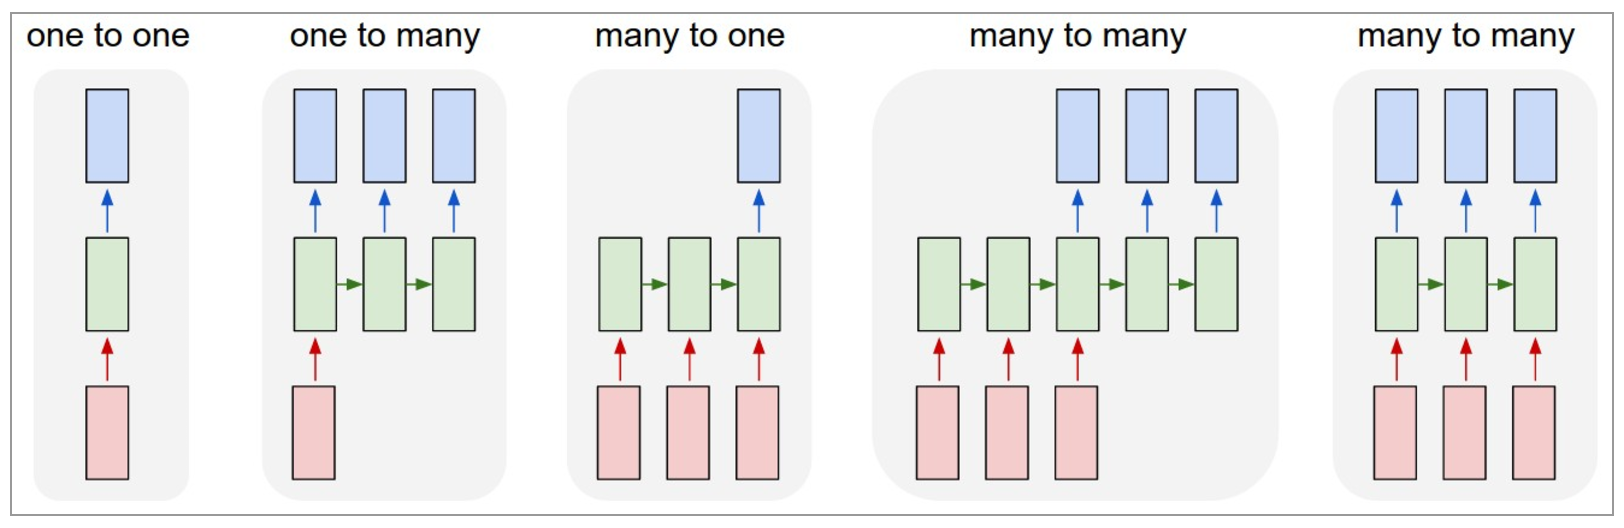
\includegraphics[width=0.9\textwidth]{img/karpathy.png}

\hfill

\url{http://karpathy.github.io/2015/05/21/rnn-effectiveness/}
\end{frame}
%

\begin{frame}{Background (LSTM/GRU and motivation for QRNN)}{}
\begin{itemize}
\item Hochreiter and Schmidhuber. 1997. LSTM.
\item Cho et al. 2014. GRU.
\end{itemize}

\begin{columns}[T] % align columns
\begin{column}{.48\textwidth}
\centering
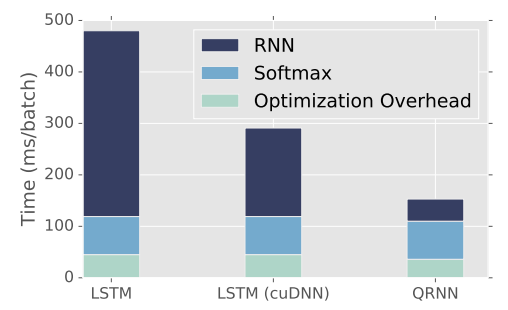
\includegraphics[width=\textwidth]{img/qrnn_perf.png}

QRNN
\end{column}%
\hfill%
\begin{column}{.48\textwidth}
\begin{minipage}[c][.4\textheight][c]{\linewidth}
\centering
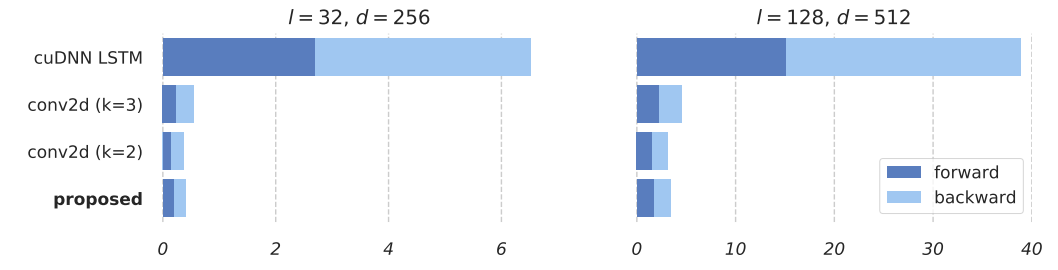
\includegraphics[width=\textwidth]{img/sru_perf.png}

SRU
\end{minipage}
\end{column}%
\end{columns}

\end{frame}

% Model: Transform Network (Encoder and Decoder)
\begin{frame}{Model: Transform Network (Encoder and Decoder)}{}
\centering
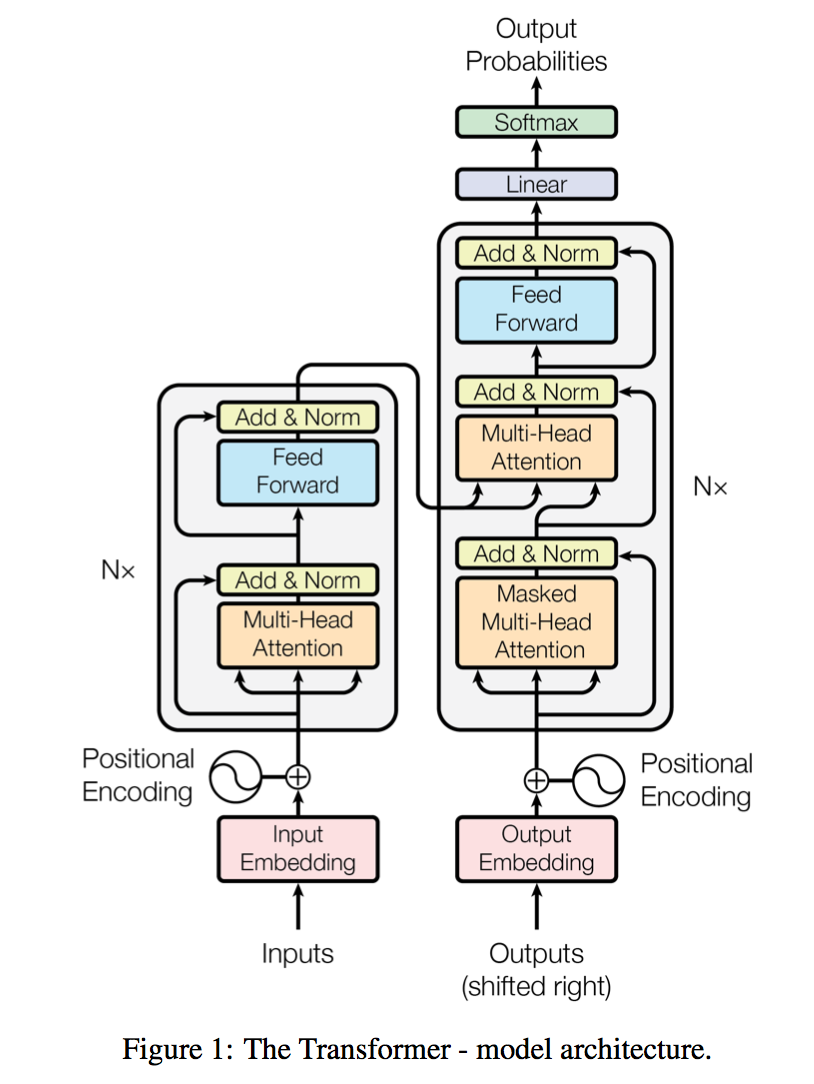
\includegraphics[width=0.5\textwidth]{img/transformer.png}
\end{frame}
%

% Scaled Dot-Product Attention
\begin{frame}[fragile]{Scaled Dot-Product Attention}{}
\begin{columns}[T] % align columns
\begin{column}{.48\textwidth}
\centering
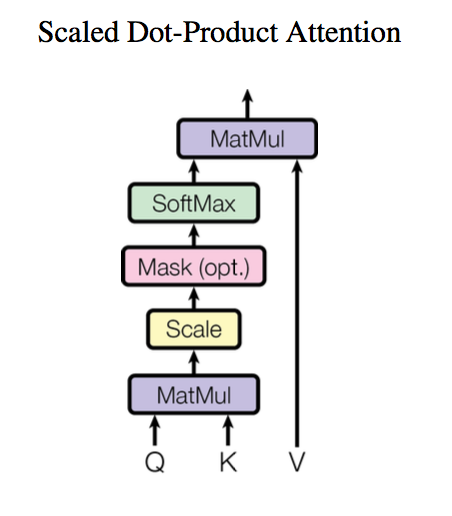
\includegraphics[width=\textwidth]{img/attn_fig.png}
\end{column}%
\hfill%
\begin{column}{.48\textwidth}
\begin{minipage}[c][.6\textheight][c]{\linewidth}
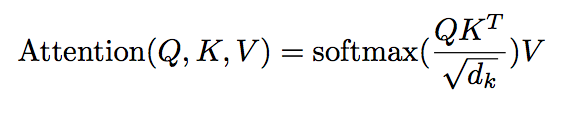
\includegraphics[width=\textwidth]{img/attn_eq.png}
\end{minipage}
\end{column}%
\end{columns}

\begin{itemize}
\item Scaling is the same as Softmax plus Temperature. Higher Temperature brings probabilities closer to uniform.
\end{itemize}
\end{frame}
%

% Scaled Dot-Product Attention (Pytorch)
\begin{frame}[fragile]{Scaled Dot-Product Attention (Pytorch)}

Serial.

\begin{verbatim}
for query in queries:
  attn = query.view(1, D) * keys.view(K, D)
  attn = attn.sum(1) / scale
  attn = softmax(attn)
\end{verbatim}

Parallel.

\begin{verbatim}
attn = queries.repeat(1, K).view(Q * K, D) * keys.repeat(Q, 1)
attn = attn.sum(1) / scale
attn = softmax(attn)
\end{verbatim}

Parallel with broadcasting.

\begin{verbatim}
attn = querys.view(Q, 1, D) * keys.view(1, K, D)
attn = attn.view(Q * K, D).sum(1) / scale
attn = softmax(attn)
\end{verbatim}
\end{frame}
%

% Multi-Head Attention
\begin{frame}{Multi-Head Attention}{}
\centering
\begin{columns}[T] % align columns
\begin{column}{.38\textwidth}
\centering
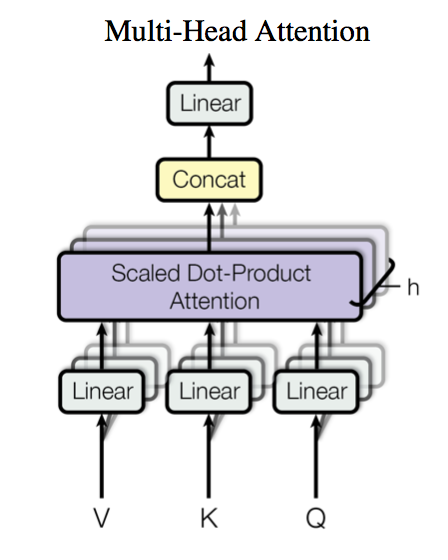
\includegraphics[width=0.6\textwidth]{img/multi_attn_fig.png}
\end{column}%
\hfill%
\begin{column}{.58\textwidth}
\begin{minipage}[c][.4\textheight][c]{\linewidth}
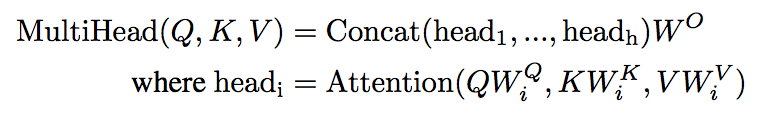
\includegraphics[width=\textwidth]{img/multi_attn_eq.png}
\end{minipage}
\end{column}%
\end{columns}

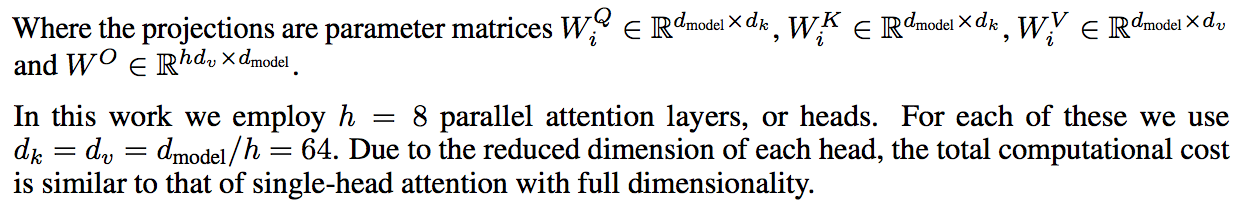
\includegraphics[width=\textwidth]{img/multi_attn_text.png}

Perform attention multiple times (almost like a dynamic attention ``kernel'').
\end{frame}
%

% Other Tricks
\begin{frame}{Other Tricks}{}
\begin{enumerate}
\item Masking in Softmax is done with $-\infty$.
\item The parameters are shared between the embedding layers \textit{and the pre-softmax layer}.
\item Positional encodings give a weak sense of ordering (similar was done in Parikh et al.).
\end{enumerate}

\begin{columns}[T] % align columns
\begin{column}{.38\textwidth}
\begin{minipage}[c][.4\textheight][c]{\linewidth}
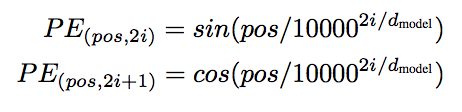
\includegraphics[width=\textwidth]{img/pos_emb.png}
\end{minipage}
\end{column}%
\hfill%
\begin{column}{.58\textwidth}
\begin{minipage}[c][.4\textheight][c]{\linewidth}
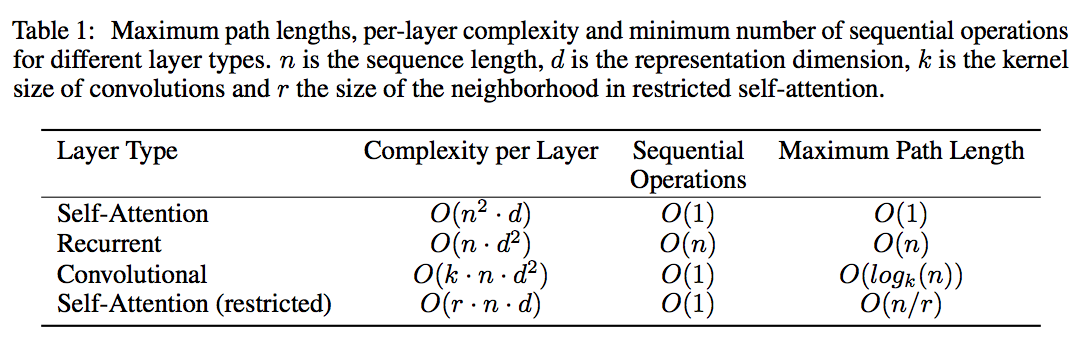
\includegraphics[width=\textwidth]{img/path_length.png}
\end{minipage}
\end{column}%
\end{columns}

\end{frame}
%

% Training
\begin{frame}{Training}{}
\begin{itemize}
\item WMT 14 (En to Ge). 4.5M pairs. BPE w. 37k vocab.
\item WMT 14 (En to Fr). 36M pairs(?). Wordpiece w. 32k vocab. 
\item Batch Size: 25k.
\item 8 GPUs (x 3584 cores; 16GB; 720GBps)
\item Small = 0.4s / step. 100k steps (12 hours). Big = 1s / step. 300k steps (3.5 days).
\item Adam with learning rate warmup and decay.
\item Regularization...

\end{itemize}
\end{frame}
%

% Training (Regularization)
\begin{frame}{Training (Regularization)}{}
\begin{itemize}
\item Residual Dropout
\item Attention Dropout
\item Label Smoothing
\item Layer Normalization \footnote[frame]{\url{https://github.com/pytorch/pytorch/issues/1959}}\footnote[frame]{Ba, Kiros, Hinton. 2016. \url{https://arxiv.org/abs/1607.06450}}
\end{itemize}
\end{frame}
%

% Results
\begin{frame}{Results: WMT}{}
\centering
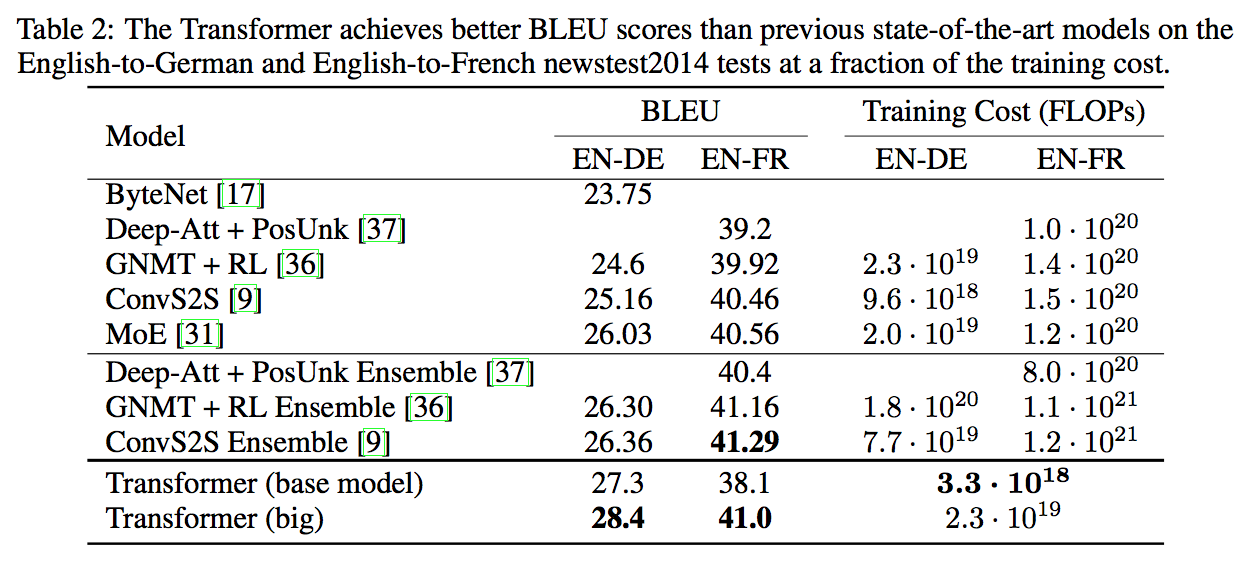
\includegraphics[width=\linewidth]{img/wmt.png}
\end{frame}
%

% Results
\begin{frame}{Results: Variations}{}
\centering
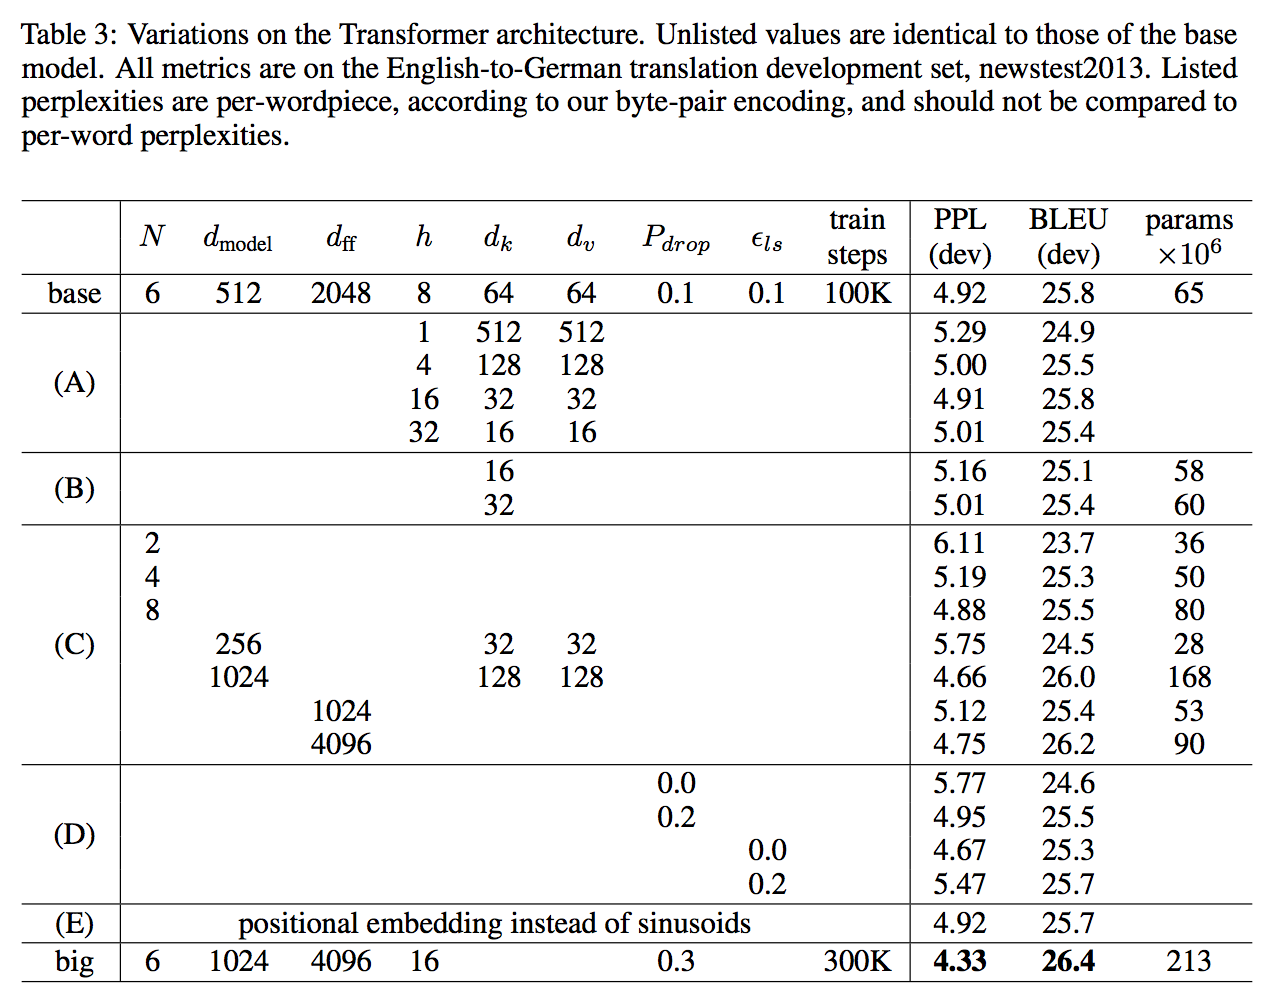
\includegraphics[width=0.8\linewidth]{img/variations.png}
\end{frame}
%

% Results
\begin{frame}{Results: PTB}{}
\centering
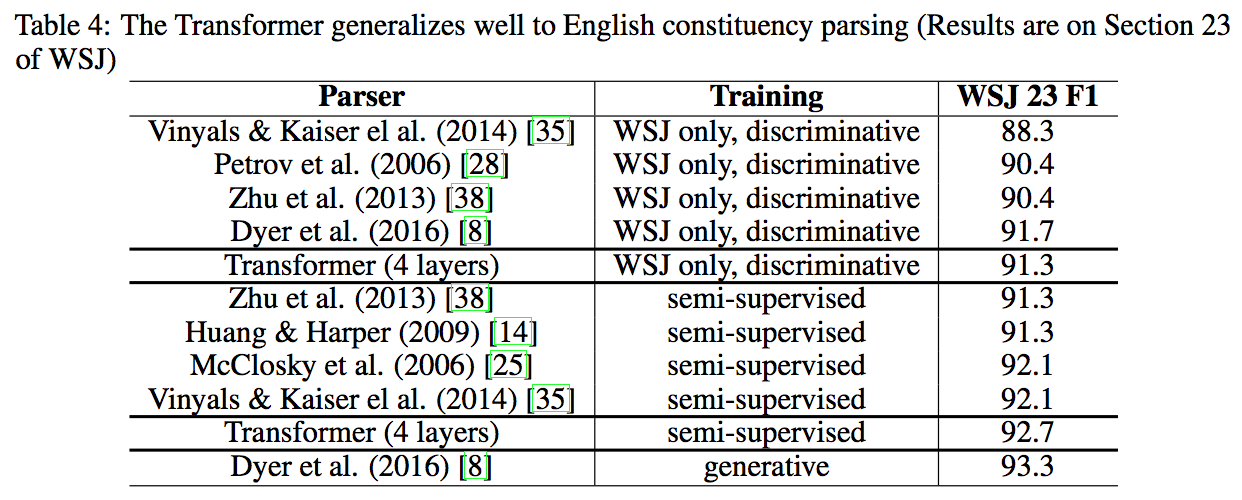
\includegraphics[width=\linewidth]{img/wsj.png}
\end{frame}
%

% Conclusion
\begin{frame}{Conclusion}{}
If you use the right tricks, you can get SotA and decrease your computational cost.
\end{frame}
%

\end{document}


